\chapter*{CARA INSTALASI APLIKASI}
\section*{\textit{INSTALASIN ANACONDA}}
\item 1.  Pertama masuk  pada browser apapun untuk mencari anaconda. Disini saya menggunakan UC Browser untuk melakukan pencariannya, Kemuadian pilih pada opsi pertama.
\begin{figure}[h]
    \centering
    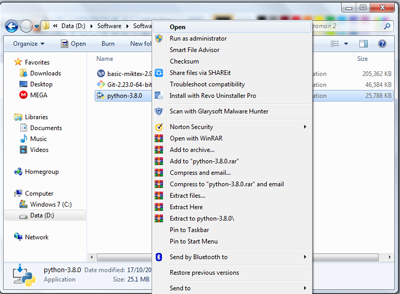
\includegraphics[scale=0.2]{gambar/1.png}
    \caption{gambar1}
    \label{fig:my_label}
\end{figure}[]
\item 2. Kemudian  setelah itu pilih button download pada pojok kiri atas sesuai gambar dibawah.
\begin{figure}[h]
    \centering
    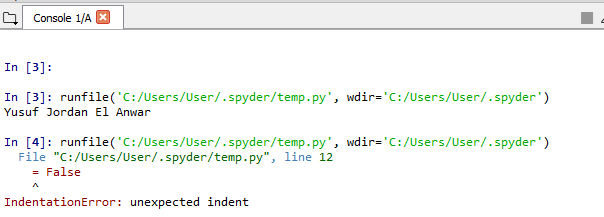
\includegraphics[scale=0.2]{gambar/2.png}
    \caption{gambar2}
    \label{fig:my_label}
\end{figure}[]
\item 3.  Setelah itu langkah selanjutnya adalah  kita memi,lik button download lagi untuk masuk ke proses selanjutnya.
\begin{figure}[h]
    \centering
    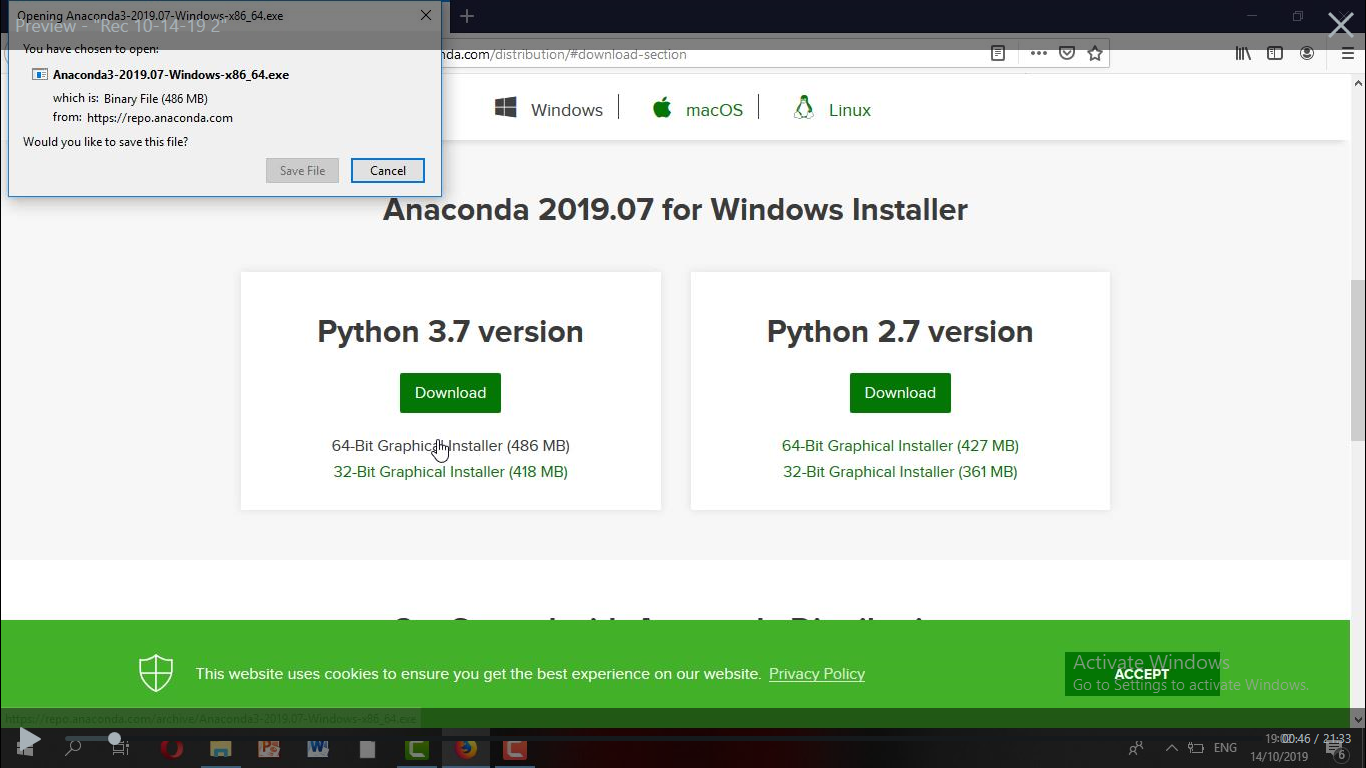
\includegraphics[scale=0.2]{gambar/3.png}
    \caption{gambar3}
    \label{fig:my_label}
\end{figure}[]
\item 4.  Selanjutnya akan muncul tampilan seperti gambar dibawah. Kemudian klik pada python  versi 3.7 lalu tekan download.
\begin{figure}[h]
    \centering
    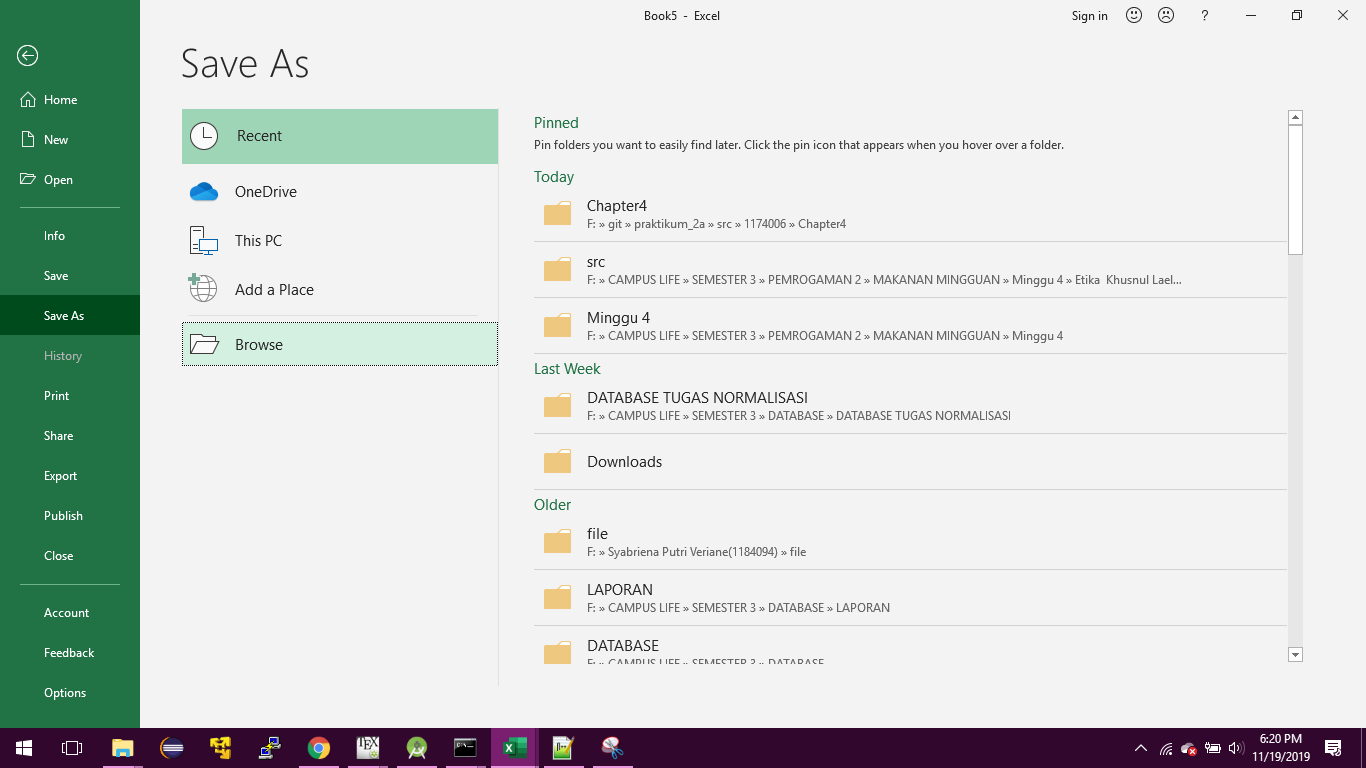
\includegraphics[scale=0.2]{gambar/4.png}
    \caption{gambar4}
    \label{fig:my_label}
\end{figure}[]
\item 5.  Langkas selanjutnya adalah kita mengeklik aplikasi anaconda kemudian tekan Run.
\begin{figure}[h]
    \centering
    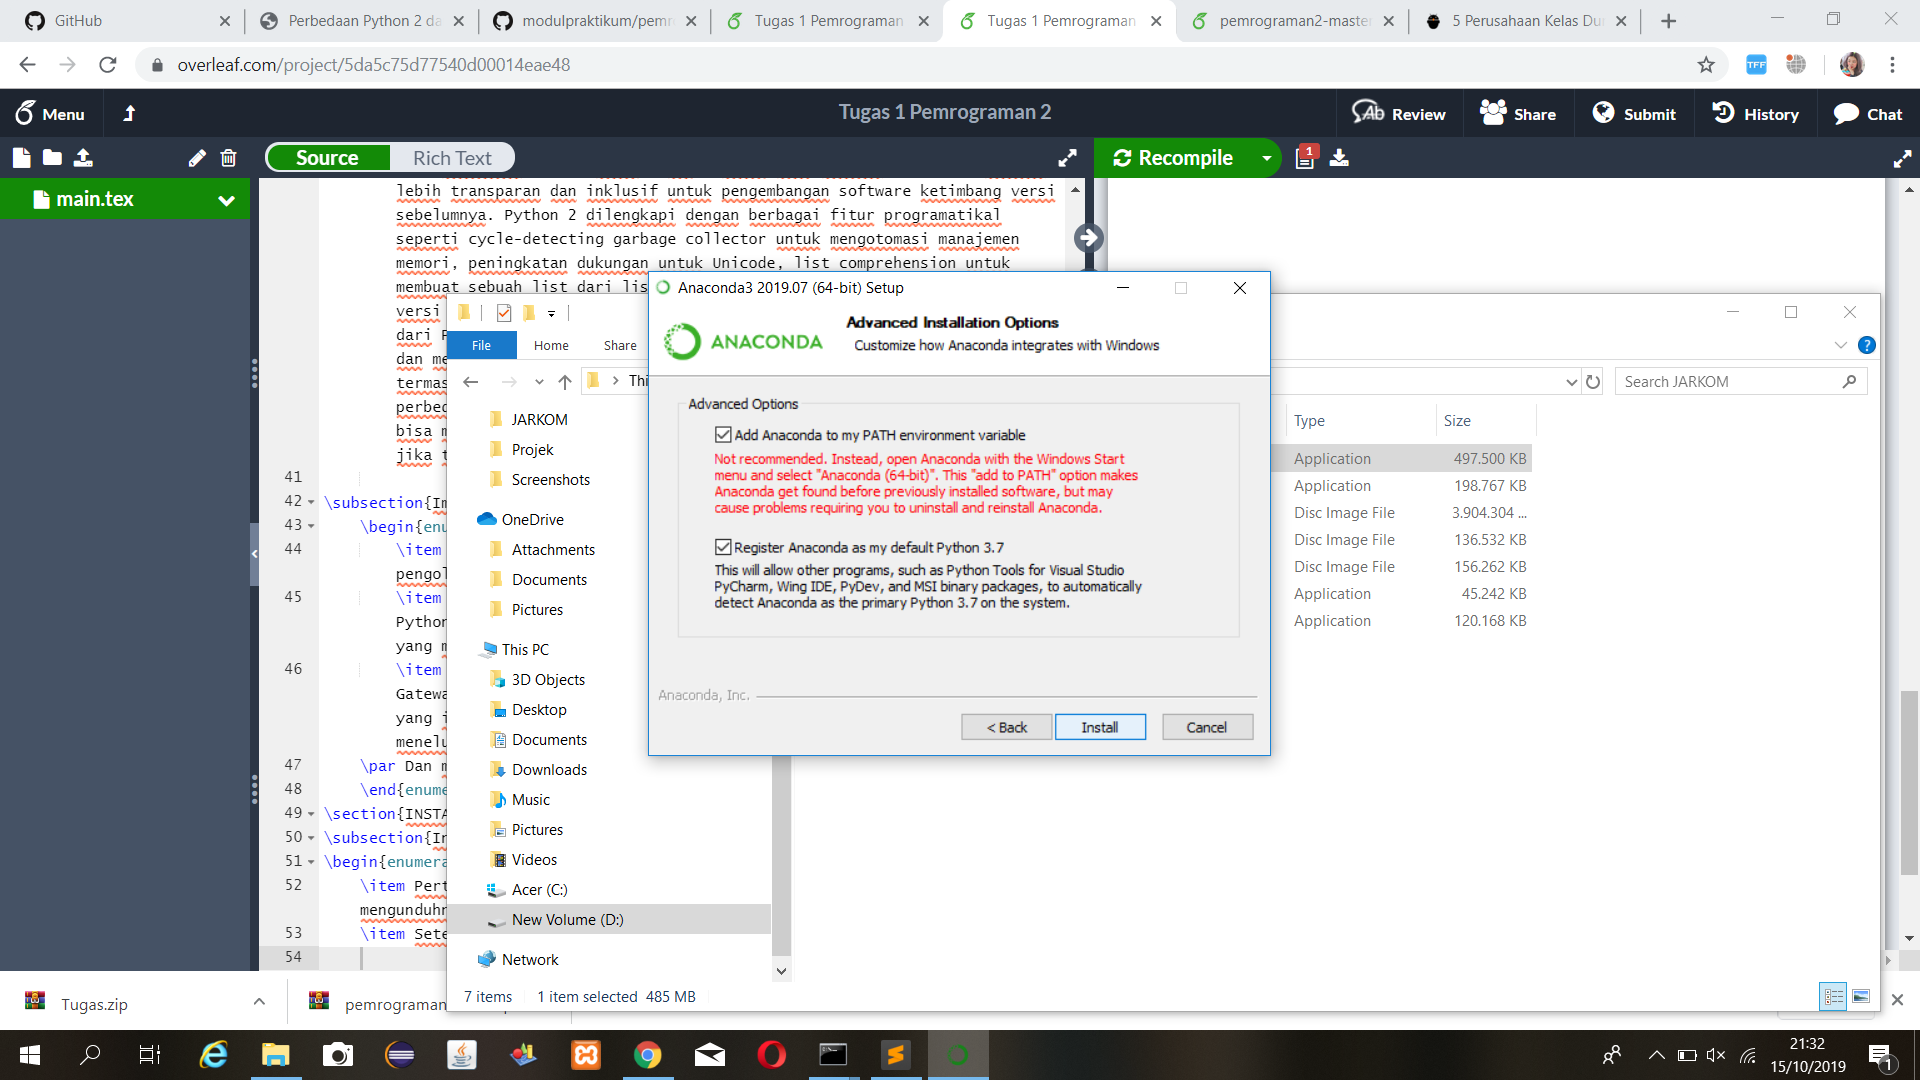
\includegraphics[scale=0.2]{gambar/5.png}
    \caption{gambar5}
    \label{fig:my_label}
\end{figure}[]
\item 6.  Pilih next untuk melanjutkan prosesnya.
\begin{figure}[h]
    \centering
    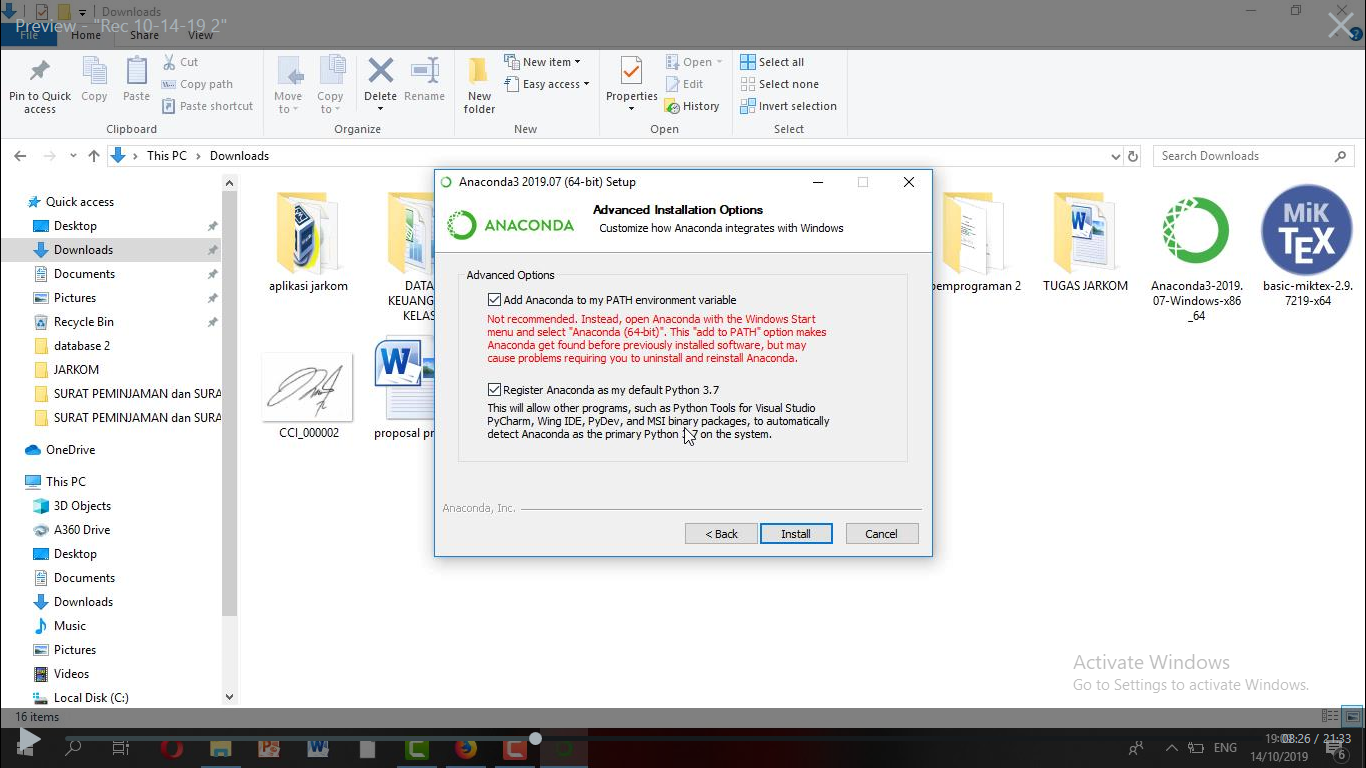
\includegraphics[scale=0.2]{gambar/6.png}
    \caption{gambar6}
    \label{fig:my_label}
\end{figure}[]
\item 7.   Selanjutnya pilih I agree untuk menjutkannya.
\begin{figure}[h]
    \centering
    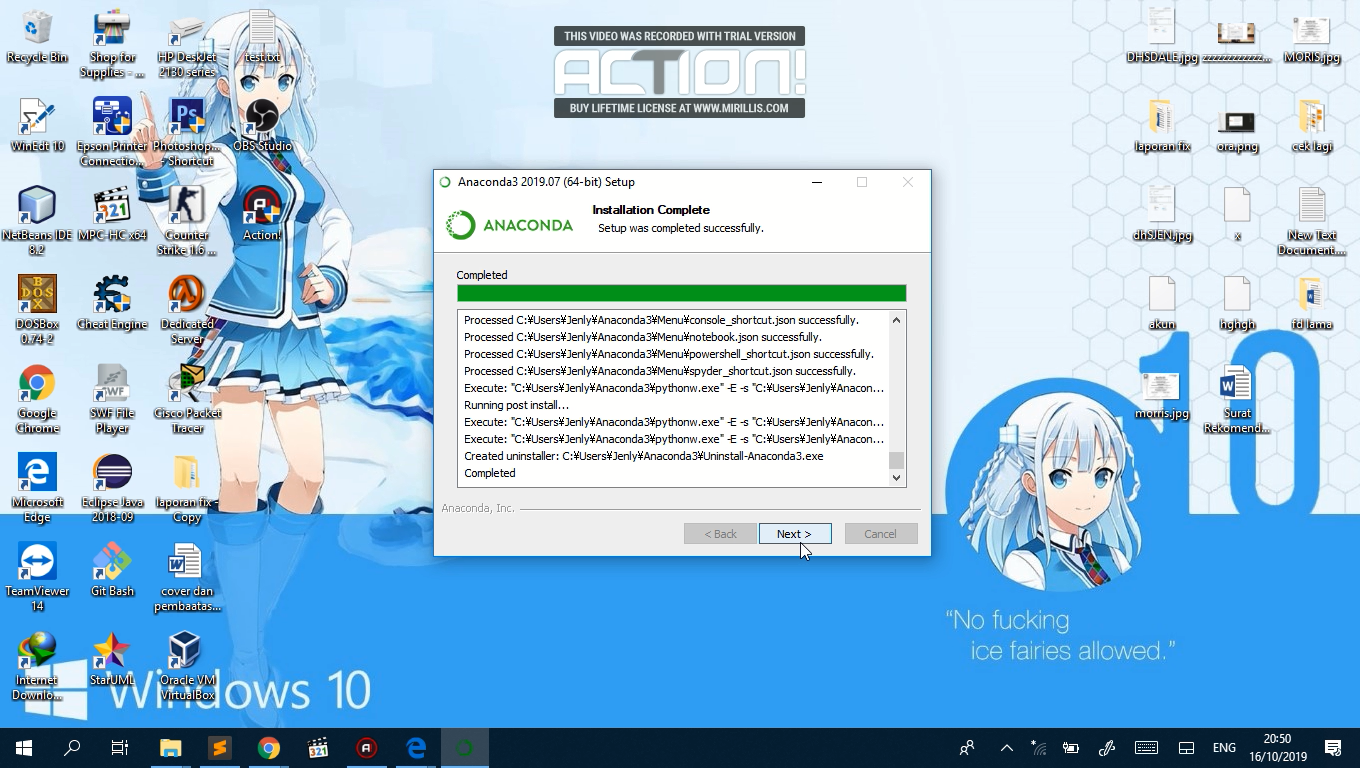
\includegraphics[scale=0.2]{gambar/7.png}
    \caption{gambar7} 
    \label{fig:my_label}
\end{figure}[]
\item 8.  Pilih opsi ‘just me’  untuk melanjutkan.
\begin{figure}[h]
    \centering
    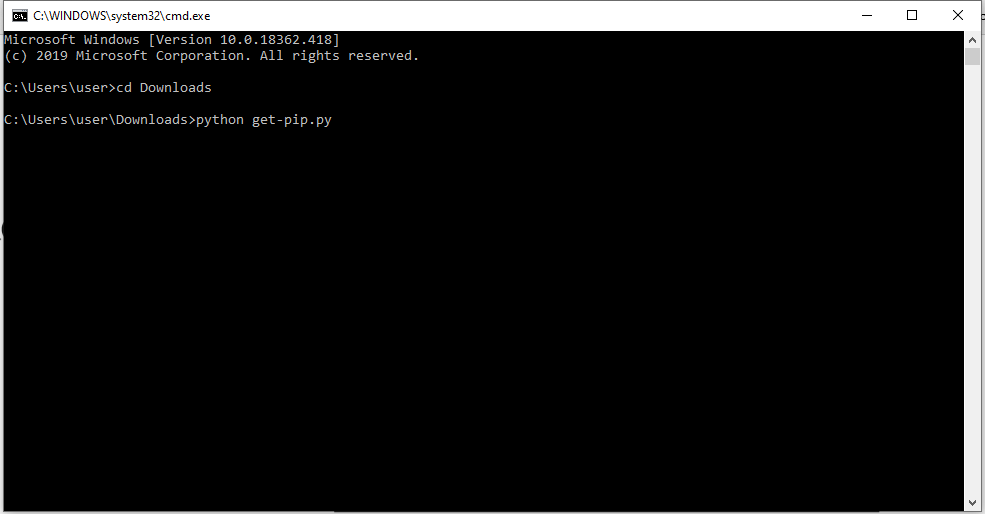
\includegraphics[scale=0.2]{gambar/8.png}
    \caption{gambar8}
    \label{fig:my_label}
\end{figure}[]
\item 9.  Lalu pilih direktori yang akan digunakan untuk menyimpanan anaconda nantinya.
\begin{figure}[h]
    \centering
    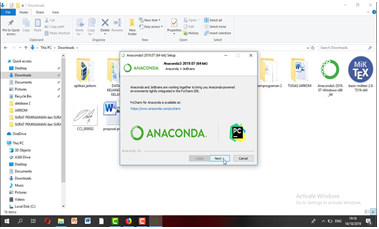
\includegraphics[scale=0.2]{gambar/9.png}
    \caption{gambar9}
    \label{fig:my_label}
\end{figure}[]
\item 10.  Kemudian centang kedua-duanya  pada tampilan tersebut, setelah itu langsung pilih install.
\begin{figure}[h]
    \centering
    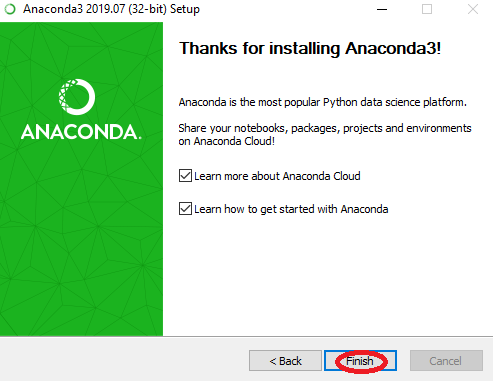
\includegraphics[scale=0.2]{gambar/10.png}
    \caption{gambar10}
    \label{fig:my_label}
\end{figure}[]
\item 11.  Tunggu sampe proses instalasinya selesai.
\begin{figure}[h]
    \centering
    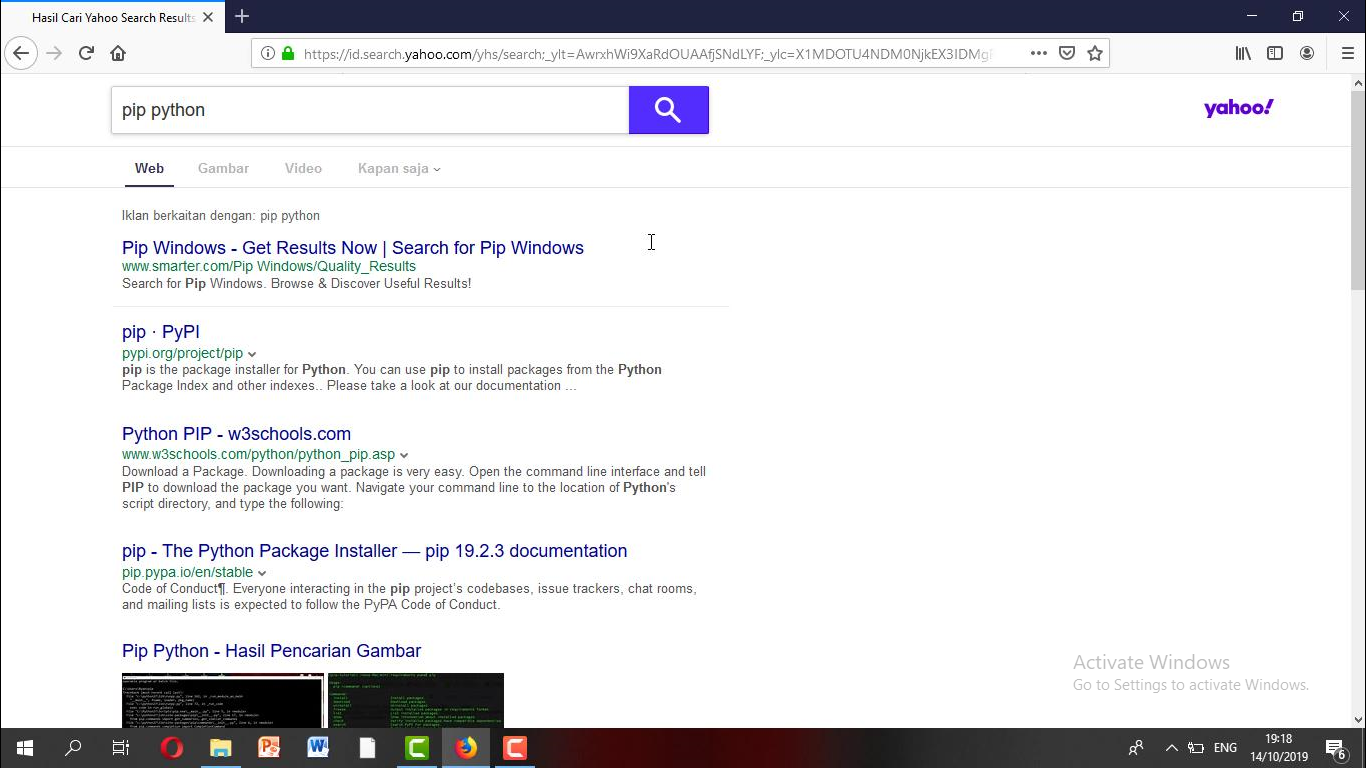
\includegraphics[scale=0.2]{gambar/11.png}
    \caption{gambar11}
    \label{fig:my_label}
\end{figure}[]
\item 12.  Setelah proses installnya selesai setelah itu pilih next untuk melanjutkan ke proses selanjutnya.
\begin{figure}[h]
    \centering
    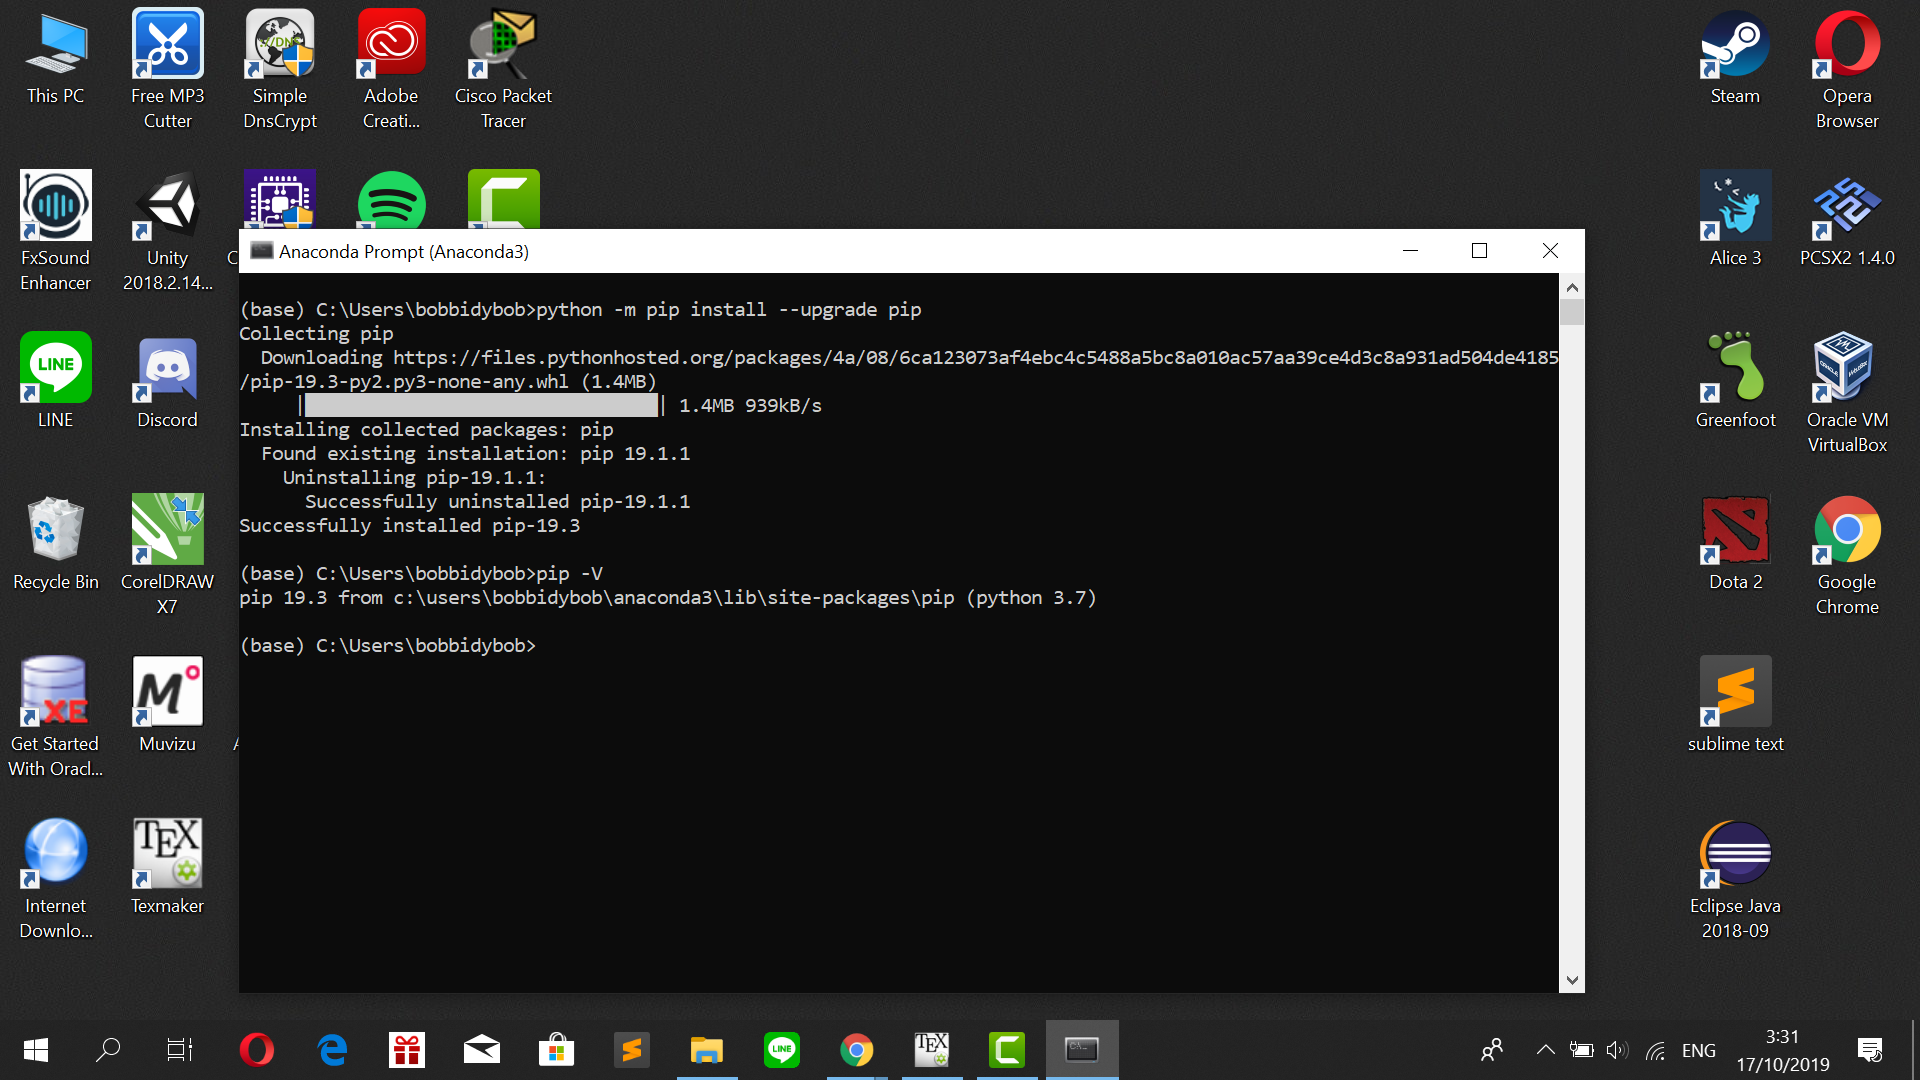
\includegraphics[scale=0.2]{gambar/12.png}
    \caption{gambar12}
    \label{fig:my_label}
\end{figure}[]
\item 13.  Pilih lagi opsi next untuk kedua kalinya untuk melanjutkan ke proses selanjutnya.
\begin{figure}[h]
    \centering
    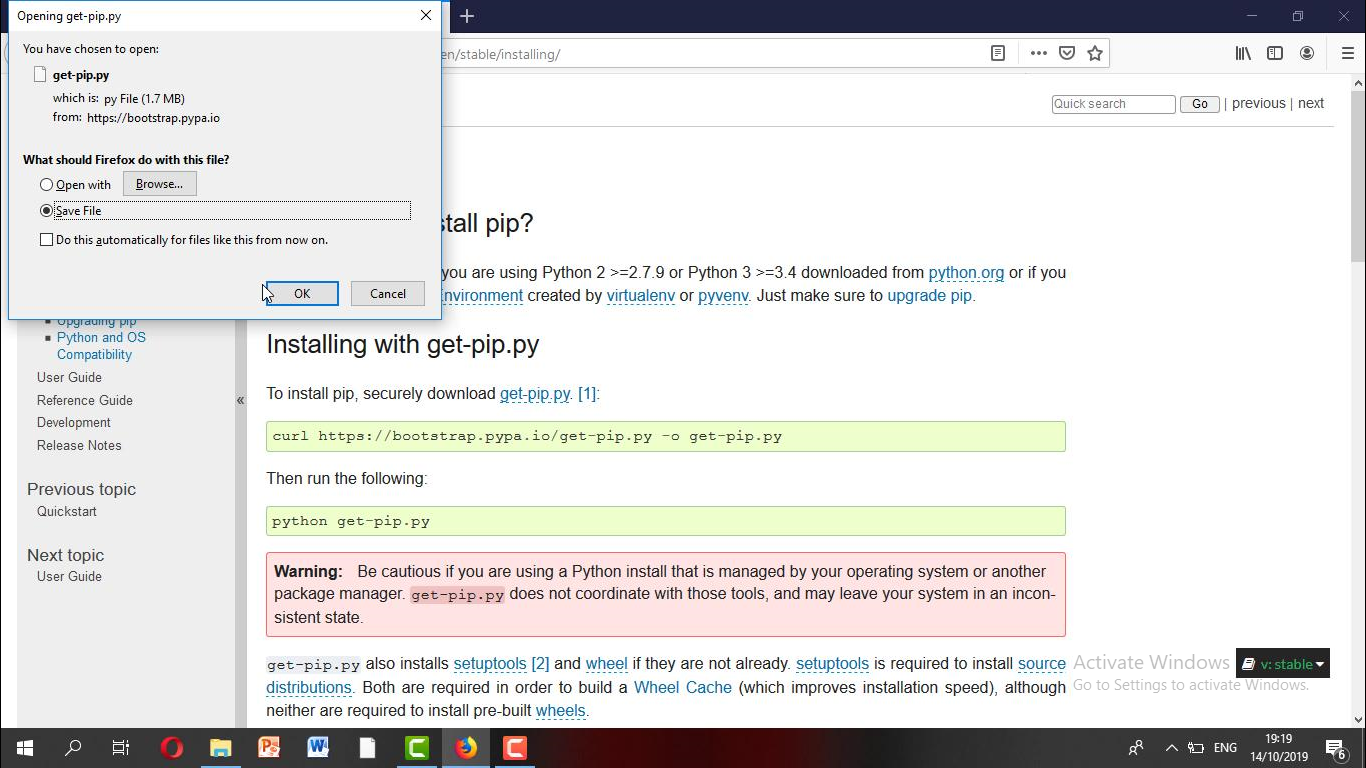
\includegraphics[scale=0.2]{gambar/13.png}
    \caption{gambar13}
    \label{fig:my_label}
\end{figure}[]
\item 14.  Terakhir proses instalasinya selesai setelah itu klik finish dan proses instalasinya selesai.
\begin{figure}[h]
    \centering
    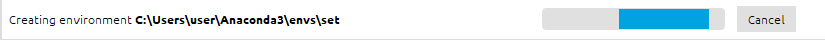
\includegraphics[scale=0.2]{gambar/14.png}
    \caption{gambar14}
    \label{fig:my_label}
\end{figure}[]


\section*{\textit{INSTALASIN PIP}}
\item 15.  Mencari pip python pada browser. Disini saya menggunakan UC Browser.
\begin{figure}[h]
    \centering
    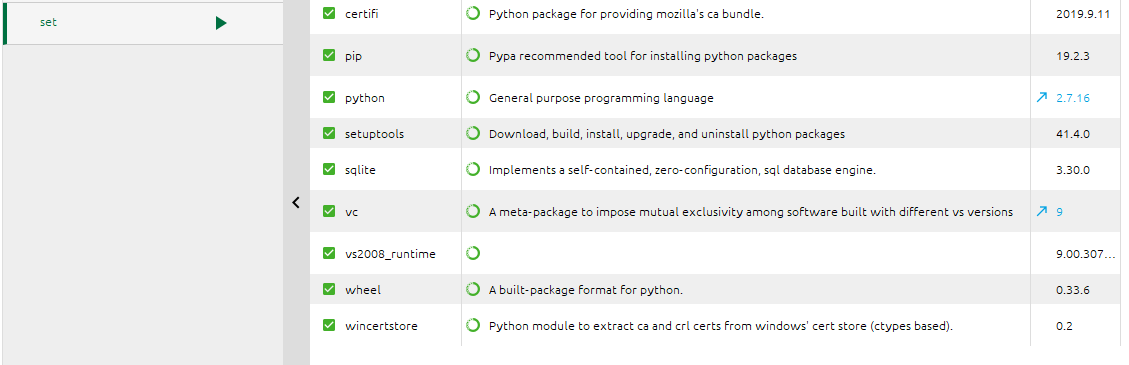
\includegraphics[scale=0.2]{gambar/15.png}
    \caption{gambar15}
    \label{fig:my_label}
\end{figure}[]
\item 16.  Kemudian pilih pada bagian pertama yaitu” pip-PyPl.
\begin{figure}[h]
    \centering
    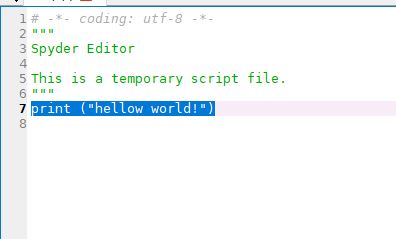
\includegraphics[scale=0.2]{gambar/16.png}
    \caption{gambar16}
    \label{fig:my_label}
\end{figure}[]
\item 17.  Kemudian kita masuk pada halaman ini lalu setelah itu pilih opsi instalation.
\begin{figure}[h]
    \centering
    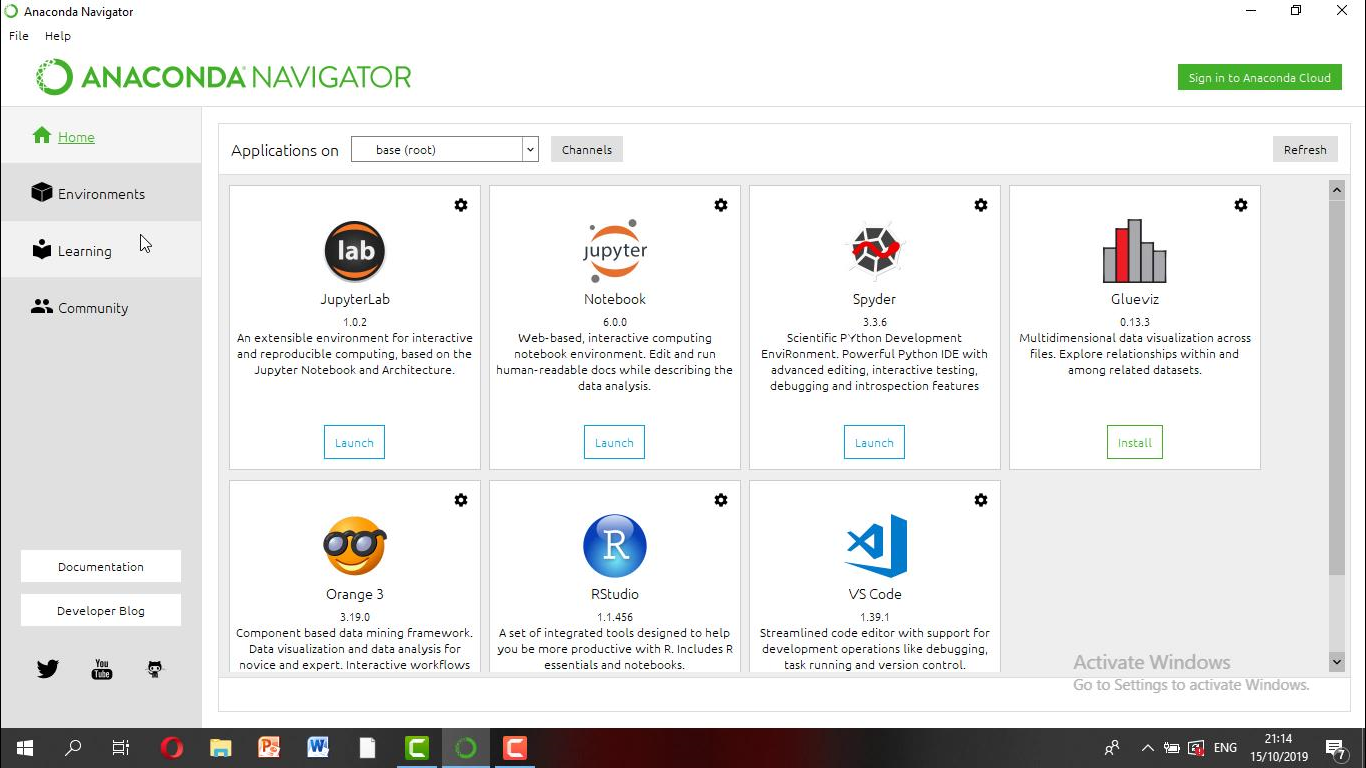
\includegraphics[scale=0.2]{gambar/17.png}
    \caption{gambar17}
    \label{fig:my_label}
\end{figure}[]
\item 18.  Kemudian pilih get-pip.py.
\begin{figure}[h]
    \centering
    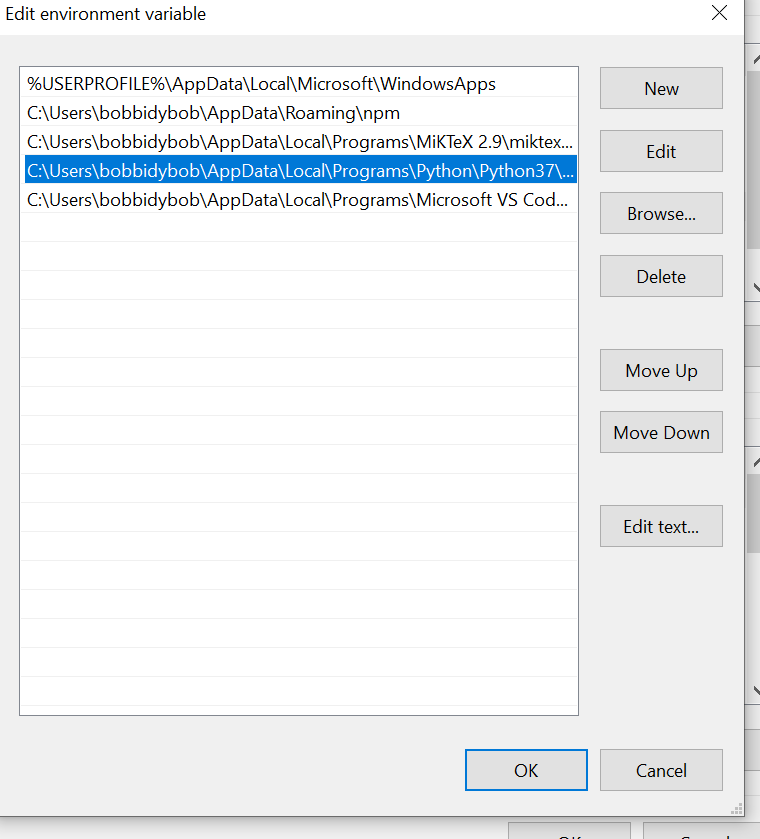
\includegraphics[scale=0.2]{gambar/18.png}
    \caption{gambar18}
    \label{fig:my_label}
\end{figure}[]
\item 19. Kemudian setelah kita mengeklik get-pip.py maka akan muncul tulisan seperti ini.
\begin{figure}[h]
    \centering
    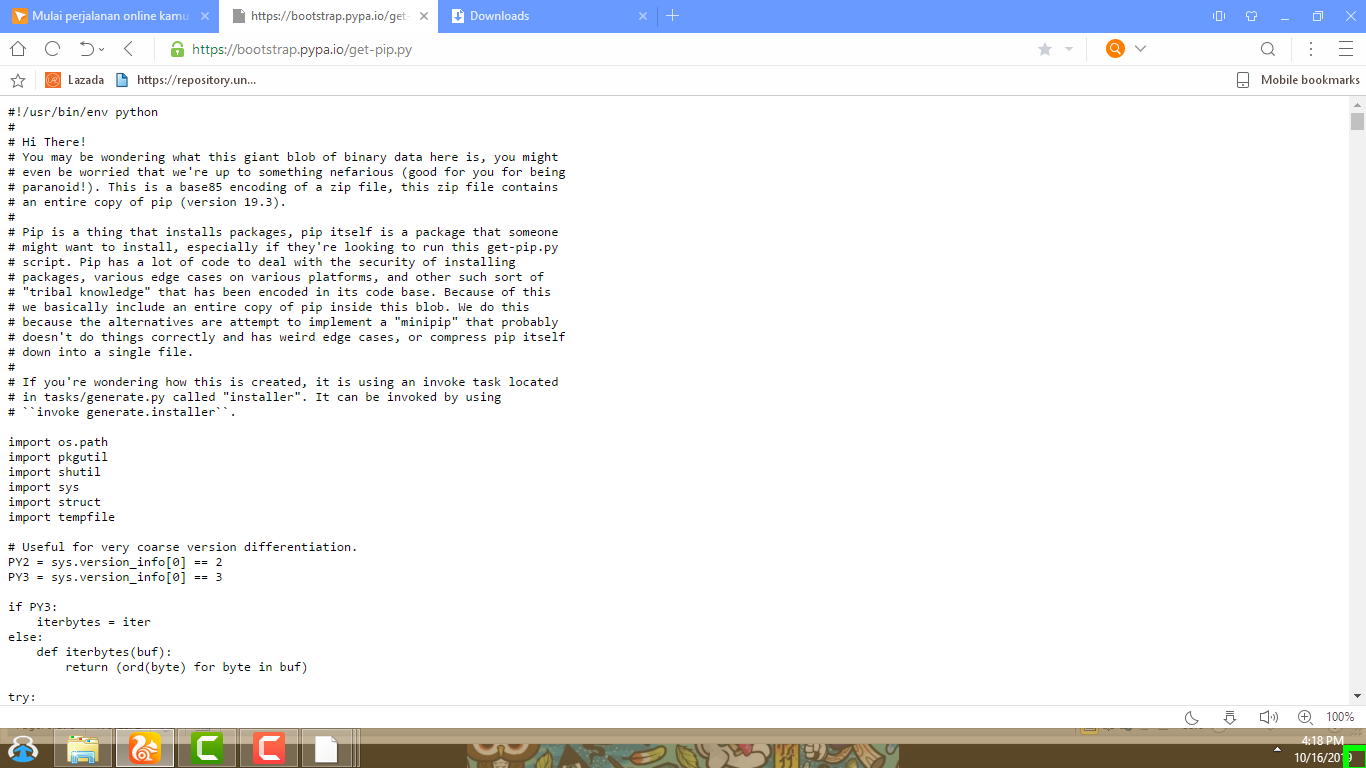
\includegraphics[scale=0.2]{gambar/19.png}
    \caption{gambar19}
    \label{fig:my_label}
\end{figure}[]
\item 20.  Kemudian kita klik pada keyboard CTRL + S maka akan keluar tampilan seperti pada gambar dibawah,setelah itu klik download.
\begin{figure}[h]
    \centering
    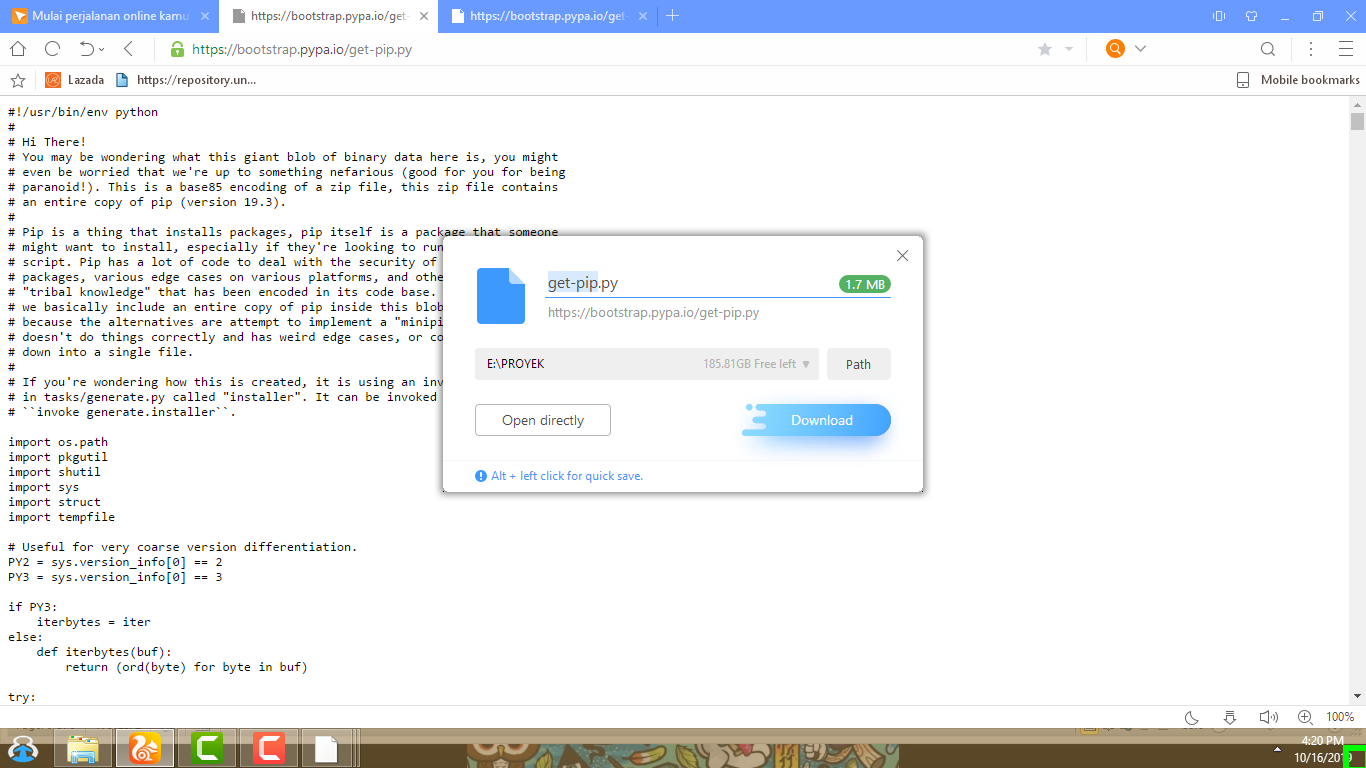
\includegraphics[scale=0.2]{gambar/20.png}
    \caption{gambar20}
    \label{fig:my_label}
\end{figure}[]
\item 21.  Kemudian setelah di download setelah itu kita masuk pada CMD untuk menginstalnya.
\begin{figure}[h]
    \centering
    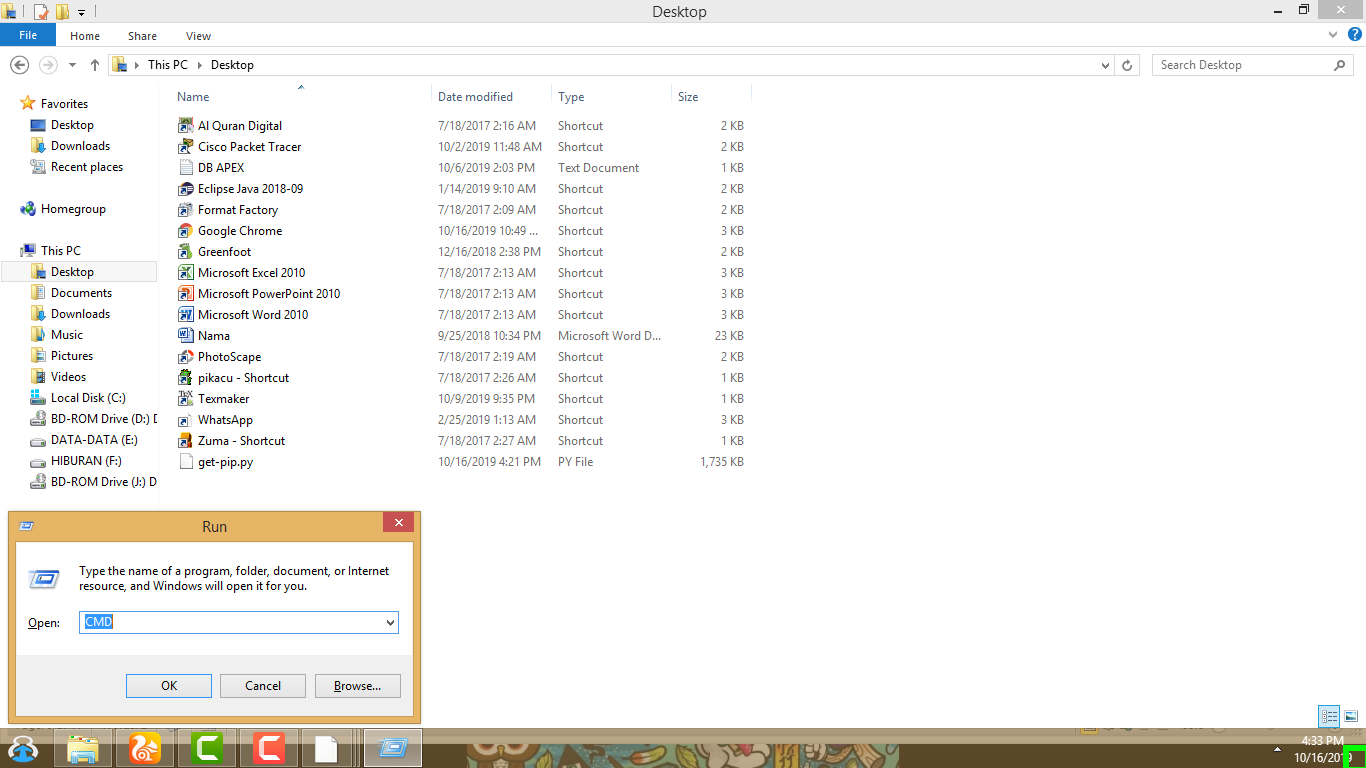
\includegraphics[scale=0.2]{gambar/21.png}
    \caption{gambar21}
    \label{fig:my_label}
\end{figure}[]
\item 22. Pertama file yang kita download tadi kita pindahin terlebih dahulu pada desktop kemudian setelah masuk pada CMD  maaka loangkah selanjutnya kita masukan kode ‘ cd Des’ kemudian tekan tab pada keyboard. Kemudian klik enter . setelah itu kita  tunggu  sampe prosesnya selesai.
\begin{figure}[h]
    \centering
    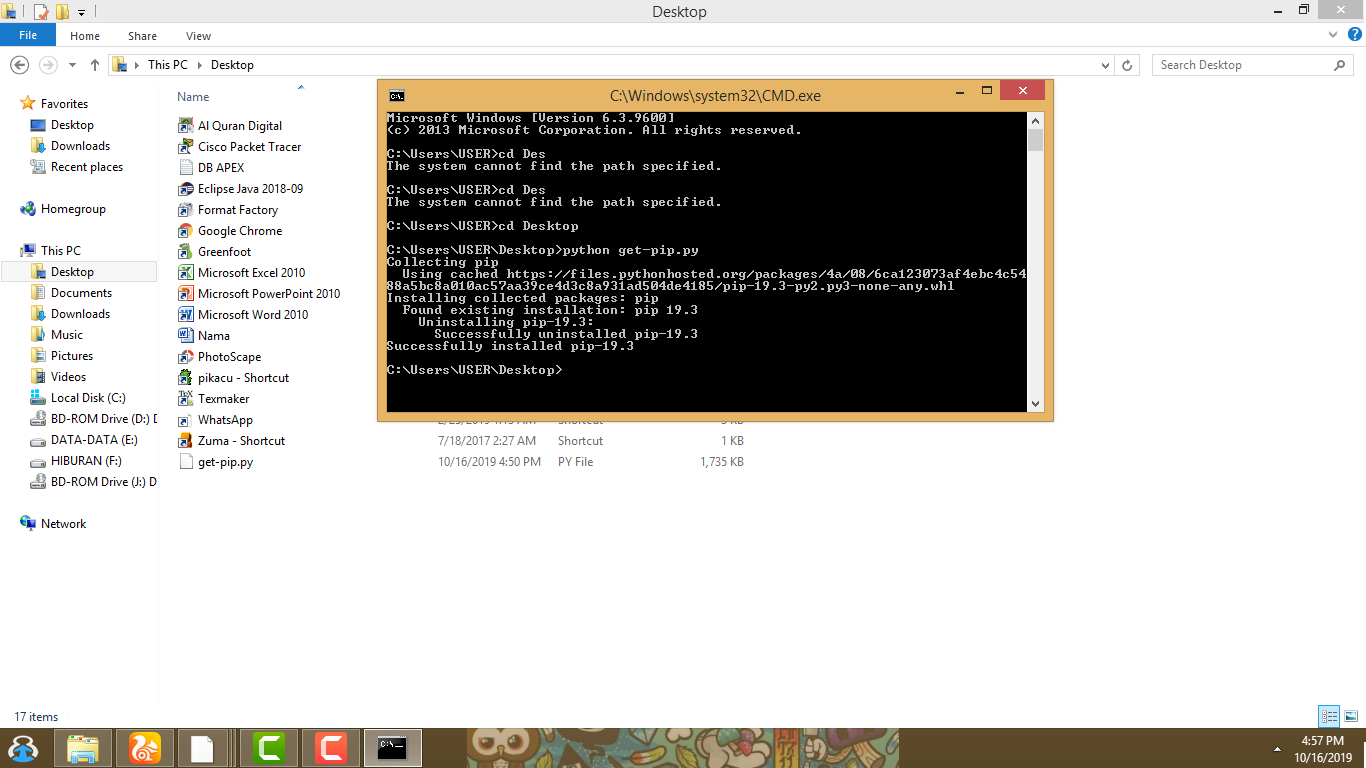
\includegraphics[scale=0.2]{gambar/22.png}
    \caption{gambar22}
    \label{fig:my_label}
\end{figure}[]

\section{MENGUPDATE ANACONDA DAN SPYDER}
\section{update anaconda}
\item 23.  Pertama kita buka CMD kemudian masukan script ‘conda install –c anaconda python setelah itu tunggu sampe proses selanjutnya.
\begin{figure}[h]
    \centering
    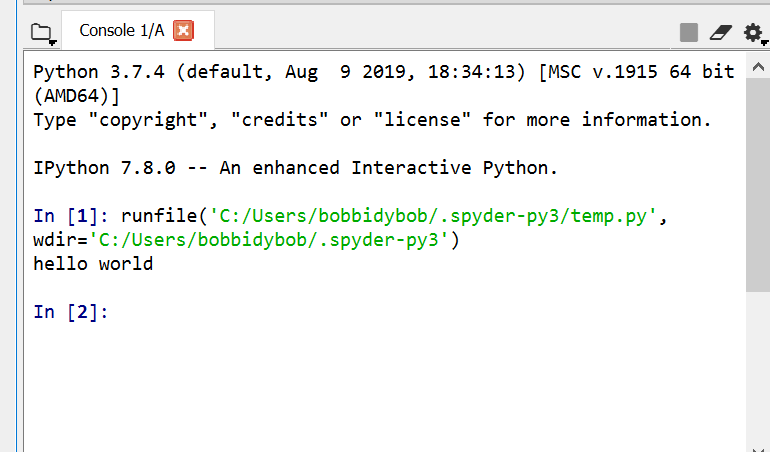
\includegraphics[scale=0.2]{gambar/23.png}
    \caption{gambar23}
    \label{fig:my_label}
\end{figure}[]
\item 24.  Kemudian langkah selanjutnya adalh kita mengetik huruf y terus enter sambil menunggu proses selanjutnya , kemudian kita ulangi proses yang seperti diawal untuk kedua kalinya.
\begin{figure}[h]
    \centering
    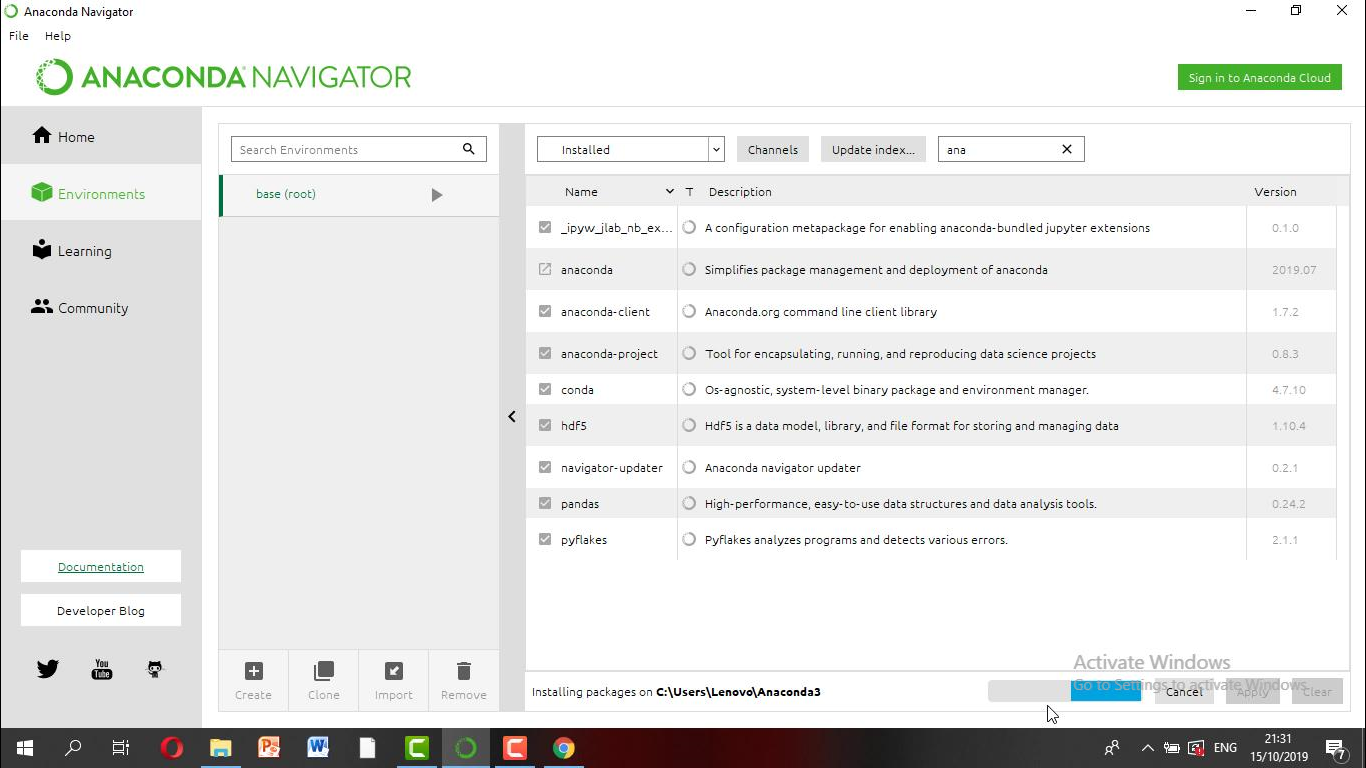
\includegraphics[scale=0.2]{gambar/24.png}
    \caption{gambar24}
    \label{fig:my_label}
\end{figure}[]
\item 25.Selanjutnya setelah proses selesai kemudian kita menulis script ‘python’ setelah prosesnya selesai maka kita selanjutnya menuliskan exit lalu setelah proses selesai kita menulis script ‘conda activate’
\begin{figure}[h]
    \centering
    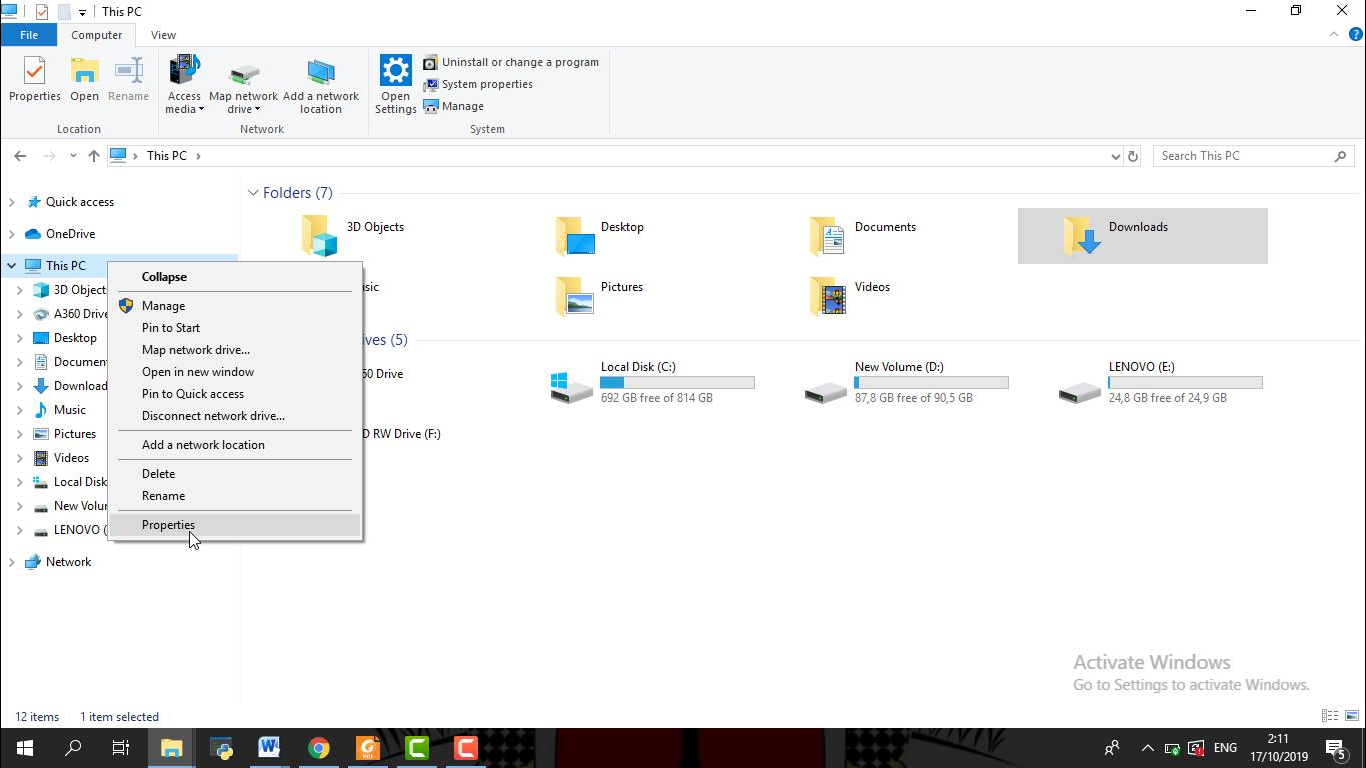
\includegraphics[scale=0.2]{gambar/25.png}
    \caption{gambar25}
    \label{fig:my_label}
\end{figure}[]
\section{update spyder}
\item 26.Pertama kita buka CMD kemudian masukan script ‘conda install –c anaconda spyder setelah itu tunggu sampe proses selanjutnya.
\begin{figure}[h]
    \centering
    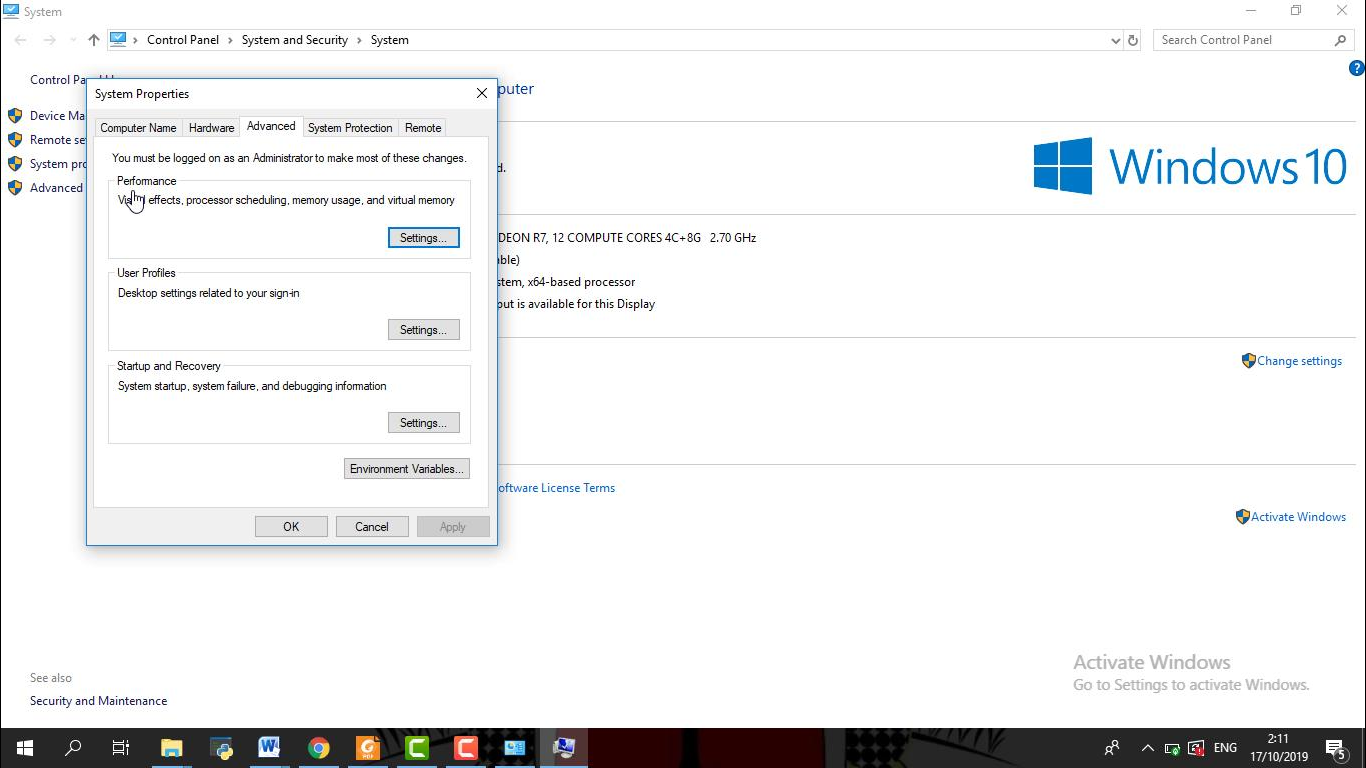
\includegraphics[scale=0.2]{gambar/26.png}
    \caption{gambar26}
    \label{fig:my_label}
\end{figure}[]
\item 27.Kemudian langkah selanjutnya adalh kita mengetik huruf y terus enter sambil menunggu proses selanjutnya , kemudian kita ulangi proses yang seperti diawal untuk kedua kalinya.
\begin{figure}[h]
    \centering
    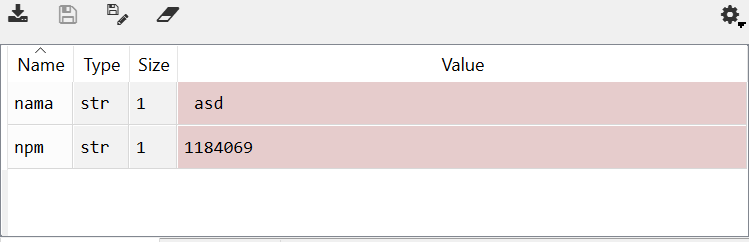
\includegraphics[scale=0.2]{gambar/27.png}
    \caption{gambar27}
    \label{fig:my_label}
\end{figure}[]
\section{MENANPILKAN SCRIPT HELLO WORLD ADA SPYDER}
\item 28.Kita menulis script print{‘hello world’} terlebih dahulu kemuadia setelah itu di run.
\begin{figure}[h]
    \centering
    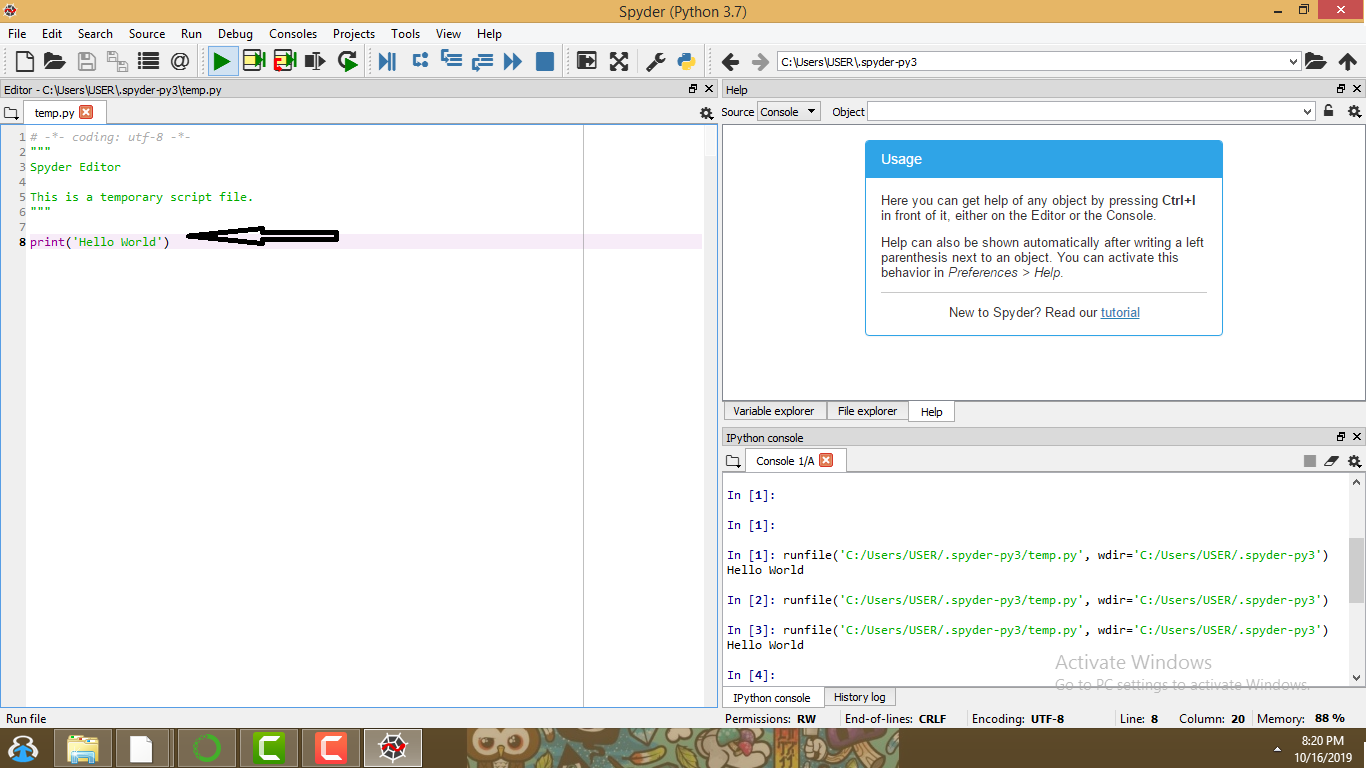
\includegraphics[scale=0.2]{gambar/29.png}
    \caption{gambar28}
    \label{fig:my_label}
\end{figure}[]
\item 29.setelah di run maka akan keluar tulisan Hello World pada samping kanan bawah.
\begin{figure}[h]
    \centering
    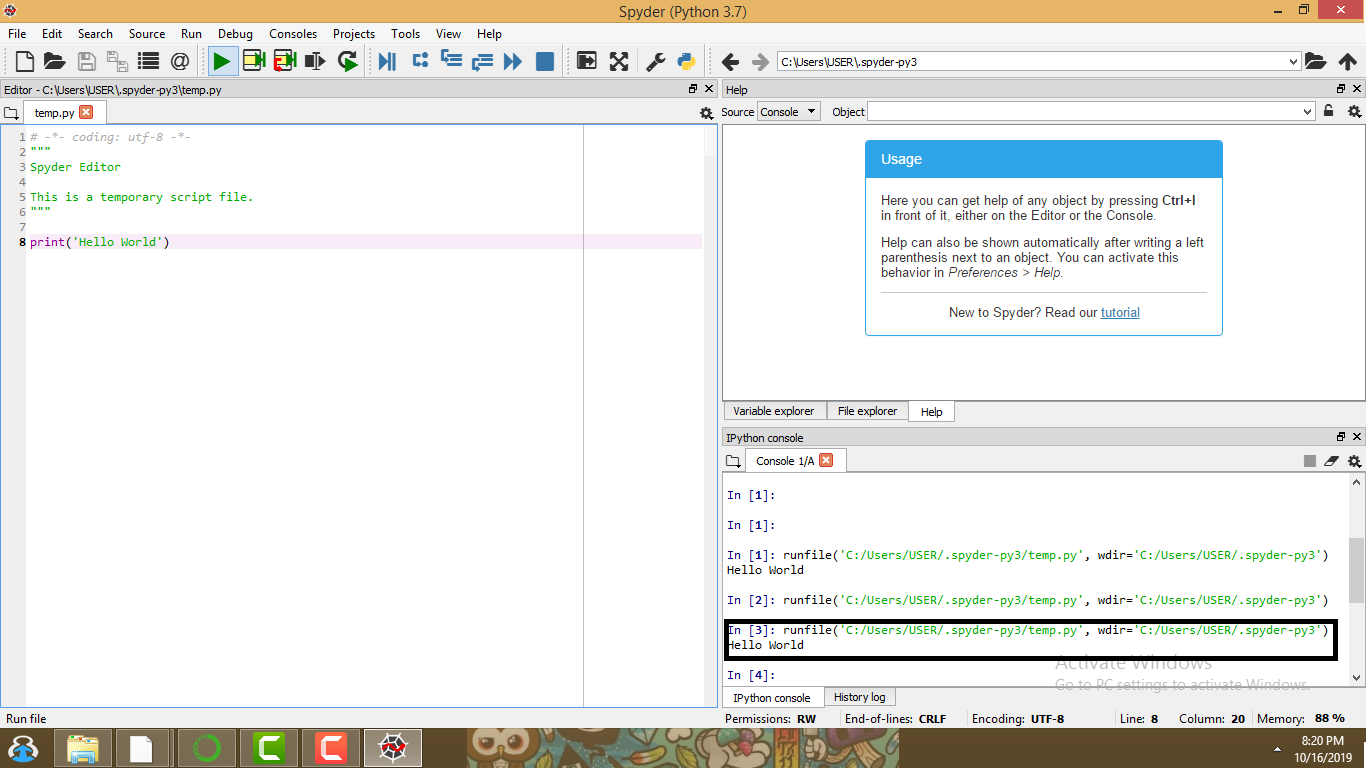
\includegraphics[scale=0.2]{gambar/30.png}
    \caption{gambar29}
    \label{fig:my_label}
\end{figure}[]




